Es folgen in diesem Abschnitt die Auswertung der Messdaten und die grafische Darstellung der selbigen.

\subsection{Direktes Beobachten}
In einem ersten Teil werden alle Messungen der direkten Beobachtung dargestellt. Es werden jeweils zwei unterschiedliche Objekte ausgemessen.

\subsubsection{Spalt}

Dieser Versuch zeigt auf wie mittels eines Laser mit bekannter Wellenlänge und einer Matscheibe die Breite eines unbekannten Spaltes ermittelt werden kann. Der dafür benötigte Aufbau ist in Kapitel \ref{sec:direkt} beschrieben. Der Abstand der resultierenden Maximas auf der Matscheibe wird ermittelt. Mit diesem Lässt sich nach der Formel \ref{eq:frauen} der Winkel $\phi$ des jeweiligen Maximas berechnen. Nun kann anhand der Formel \ref{eq:spalt} eine Fittfunktion an die Messwerte, wie in Abbildung \ref{fig:messung_1_1} und \ref{fig:messung_1_2} zu sehen, angelegt.

%%%%%%%%%%%%%%%%%%%%%%%%%%%%%%%%%%%%%%%%%%%%%%%%%%%%%%%%%%%%%%%%%%%%%%%%%%%%%
\begin{figure}[htb]
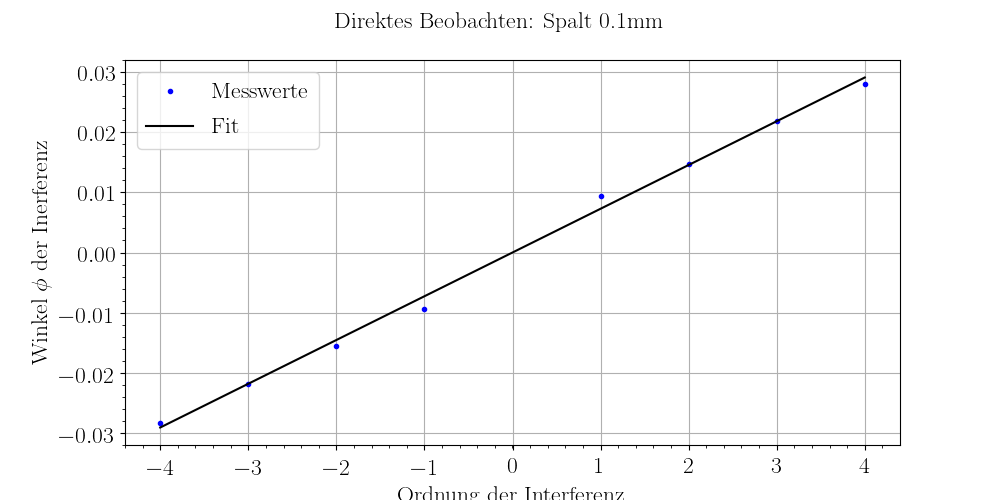
\includegraphics[width=\textwidth]{graphics/messung_1_1.png}
\caption{Winkel der Interferenzmaximas an einem Spalt 0.1mm in Abhängigkeit der Interferenzordung. Gemessen auf einer Mattscheibe. Distanz Messobjekt zu Mattscheibe beträgt 234.4cm. Verwendeter Laser ist ein He-Ne-Laser mit einer Wellenlänge von 632.8nm} % picture caption
\label{fig:messung_1_1}
\end{figure}
%%%%%%%%%%%%%%%%%%%%%%%%%%%%%%%%%%%%%%%%%%%%%%%%%%%%%%%%%%%%%%%%%%%%%%%%%%%%%

Für die Spaltbreite $b$ wurde folgender Fitwert berechnet: $\underline{86\pm 2\mu m}$
\newpage


%%%%%%%%%%%%%%%%%%%%%%%%%%%%%%%%%%%%%%%%%%%%%%%%%%%%%%%%%%%%%%%%%%%%%%%%%%%%%
\begin{figure}[htb]
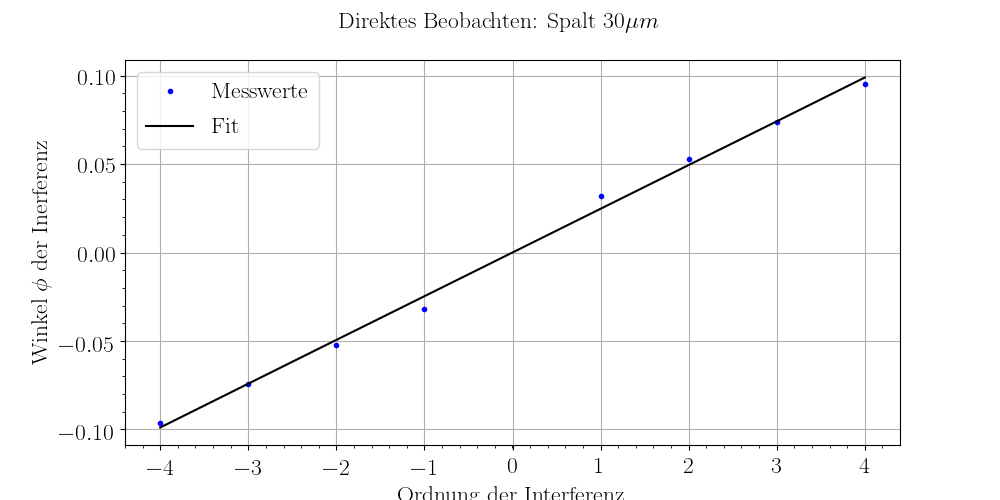
\includegraphics[width=\textwidth]{graphics/messung_1_2.png}
\caption{Winkel der Interferenzmaximas an einem Spalt $30\mu m$ in Abhängigkeit der Interferenzordung. Gemessen auf einer Mattscheibe. Distanz Messobjekt zu Mattscheibe beträgt 234.4cm. Verwendeter Laser ist ein He-Ne-Laser mit einer Wellenlänge von 632.8nm} % picture caption
\label{fig:messung_1_2}
\end{figure}
%%%%%%%%%%%%%%%%%%%%%%%%%%%%%%%%%%%%%%%%%%%%%%%%%%%%%%%%%%%%%%%%%%%%%%%%%%%%%

Für die Spaltbreite $b$ wurde folgender Fitwert berechnet: $\underline{25.6 \pm 0.6\mu m}$
